\documentclass[a4paper]{article}
%\documentclass[twocolumn]{article}

\usepackage{graphicx}
\usepackage{listings}
\usepackage{xcolor}
%\usepackage{enumitem}
\usepackage{enumerate}
\usepackage{CJKutf8} %注意这里用的是CJKutf8而不是CJK
\usepackage{indentfirst}

\usepackage{tikz} % 画流程图用的
\usepackage{qtree}
\usepackage{indentfirst}%英文首行缩进
\usepackage{fancyhdr} % 排版格式
\usepackage{hyphenat} % 单词断字
\usepackage{amsmath} % for {aligned}, 公式换行
\usepackage{multicol}% 多栏排版
\usepackage{balance}% 双栏最后一页对齐
\usepackage{subfigure}% 多图
\usepackage{booktabs}% 表格画线,\toprule, \midrule, \bottomrule
\usepackage{ulem}
%\usepackage{clrscode}

% in texlive-science
\usepackage{algorithm}
\usepackage{algpseudocode}% an improvement from algorithmicx for algorithmic

\usepackage{setspace}

\usepackage[utf8]{inputenc}


\usepackage{xspace}

%======= XXX 要编译两遍才能有标签和引用等效果 =====%

\usepackage[top=2.54cm,bottom=2.54cm,left=3.17cm,right=3.17cm]{geometry} % a4paper standard
\usepackage[unicode=true]{hyperref} %注意这里不能加CJKbookmarks=true,否则会乱码
\usetikzlibrary{arrows,decorations.pathmorphing,backgrounds,positioning,fit,automata,trees}

\hypersetup{
    pdfauthor={ouoline},
    %pdftitle={test},
    %pdfsubject={Subject},
    %pdfkeywords={Keyword1, Keyword2, ...},
    %pdfcreator={LaTeX with hyperref package},
    %pdfproducer = {dvips + ps2pdf},
    %bookmarksnumbered=true,
    %colorlinks=no,
    pdfborder={0 0 0},
    %bookmarksopen=true,
}
%------------------------------------------------------------------%

\setcounter{secnumdepth}{5} % 编号的深度,4 表示到 paragraph 一级
%\setcounter{tocdepth}{4} % 目录中的深度

%------------------------------------------------------------------%
\usepackage{color}
\definecolor{lightgray}{rgb}{.9,.9,.9}
\definecolor{darkgray}{rgb}{.4,.4,.4}
\definecolor{purple}{rgb}{0.65, 0.12, 0.82}

\lstdefinelanguage{JavaScript}{
  keywords={typeof, new, true, false, catch, function, return, null, catch, switch, var, if, in, while, do, else, case, break},
  keywordstyle=\color{blue}\bfseries,
  ndkeywords={class, export, boolean, throw, implements, import, this},
  ndkeywordstyle=\color{darkgray}\bfseries,
  identifierstyle=\color{black},
  sensitive=false,
  comment=[l]{//},
  morecomment=[s]{/*}{*/},
  commentstyle=\color{purple}\ttfamily,
  stringstyle=\color{red}\ttfamily,
  morestring=[b]',
  morestring=[b]"
}

\lstset{% general command to set parameter(s)
        language={JavaScript},
        %numbers=left,
        basicstyle=\tt, % 默认对所有字符使用等宽字体
        keywordstyle=\color{blue},%\bfseries\underbar% underlined bold black keywords
        identifierstyle=,           % nothing happens
        stringstyle=\color{purple},
        commentstyle=\color{gray},
        escapechar=`,
        showstringspaces=false,     % no special string spaces
        breaklines=true, % 自动换行
    }


%------------------------------------------------------------------%

% 自己定义新命令,参数依次是
% \newcommand{新命令名称(带反斜线)}[参数个数(最多9个)]{命令定义}
% 实际上相当于宏替换
% \newcommand{\sayhelloto}[1]{hello,#1}
\newcommand{\template}[3] {
    \item \textbf{#1}
    \begin{enumerate}
        \item[\textbf{#2}] #3
    \end{enumerate}
}
\newcommand{\jie}[2]{\template{#1}{解}{#2}}
\newcommand{\zheng}[2]{\template{#1}{证明}{#2}}

%------------------------------------------------------------------%

% 放在导言区,设置全局行距
\linespread{1.6}

% 放在导言区,公式编号和章节相关
%\makeatletter % `@' now normal ``letter''
%\@addtoreset{equation}{section}
%\makeatother % `@' is restored as ``non-letter''
%\renewcommand\theequation{\oldstylenums{\thesection}%
%.\oldstylenums{\arabic{equation}}}


\begin{document}

\begin{CJK*}{UTF8}{gbsn}
    \CJKindent
    \setlength{\parindent}{2em} % no indent

    \pagestyle{fancy}

    %\begin{center}
    %\Huge{title}
    %\vspace{25pt} % 25pt between title and text
    %\end{center}
    \title{\huge{计算机与网络体系结构(2)}\\\Large{编译原理}\\{\large 简单编译器的实现:将C语言编译为LLVM}}
    \author{
    软件11\hspace{10pt}陈 璐\hspace{10pt}2011013249\\
    软件12\hspace{10pt}王肖佑\hspace{10pt}2011013273\\
    软件11\hspace{10pt}陈华榕\hspace{10pt}2011013236
    }
    \date{\today}
    \maketitle
    \tableofcontents
    \newpage

    \section{实验背景}
    \subsection{实验环境}
    如需复现实验结果请准备一台PC机并安装Windows/OS X/Linux等桌面系统,然后安装$>=0.10.24$版本的\textit{Node}。
    \par 如需将实验结果编译为可执行程序,需要一台PC机并安装Linux桌面系统,同时通过\textit{apt-get}安装最新版本的\textit{clang}。

    \subsection{目录结构}
{
\tikzstyle{every node}=[draw=black,thick,anchor=west]
\tikzstyle{selected}=[draw=red,fill=red!30]
\tikzstyle{optional}=[dashed,fill=gray!50]
\begin{tikzpicture}[%
  grow via three points={one child at (0.5,-0.7) and
  two children at (0.5,-0.7) and (0.5,-1.4)},
  edge from parent path={(\tikzparentnode.south) |- (\tikzchildnode.west)}]
  \node {C2LLVM}
    child { node [optional] {source $|$ 源码}
        child { node [optional] {C2LLVM}
            child { node [optional] {lib $|$ 库文件}
                child { node [optional] {parser $|$ 词法语法分析器}
                    child { node {parser-entry.js $|$ 分析器类CParser}}
                    child { node {SimpleCv4.g $|$ 语法文件}}
                    child { node {SimpleCv4.tokens $|$ 语法的Token文件}}
                    child { node {SimpleCv4Lexer.js $|$ 词法分析}}
                    child { node {SimpleCv4Parser.js $|$ 语法分析}}
                }
                child [missing] {}
                child [missing] {}
                child [missing] {}
                child [missing] {}
                child [missing] {}
                child { node [optional] {inspector $|$ 语法语义检查器}
                    child { node {id-inspector.js $|$ 变量作用域检查}}
                }
                child [missing] {}
                child { node [optional] {generator $|$ 目标代码生成器}
                    child { node {LLVM.js $|$ 生成LLVM代码}}
                }
                child [missing] {}
                child { node {antlr-3.3.jar $|$ ANTLR分析工具}}
                child { node {errmgr.js $|$ 错误管理器,保存错误信息,格式化输出}}
                child { node {compiler.js $|$ Compiler类}}
            }
            child [missing] {}
            child [missing] {}
            child [missing] {}
            child [missing] {}
            child [missing] {}
            child [missing] {}
            child [missing] {}
            child [missing] {}
            child [missing] {}
            child [missing] {}
            child [missing] {}
            child [missing] {}
            child [missing] {}
            child { node [optional] {tests $|$ 自动化测试}
                child { node [optional] {data $|$ 测试数据}
                    child { node {arraylist.c $|$ 测试文件}}
                    child { node {arraylist.ll $|$ 使用clang编译为LLVM的结果}}
                }
                child [missing] {}
                child [missing] {}
                child { node [selected] {test-main.js $|$ 测试执行入口,可通过npm调用}}
            }
            child [missing] {}
            child [missing] {}
            child [missing] {}
            child [missing] {}
            child { node {index.js $|$ 库入口}}
            child { node {... $|$ 其他文件,包括定义库的package.json等}}
        }
    }
    child [missing] {}
    child [missing] {}
    child [missing] {}
    child [missing] {}
    child [missing] {}
    child [missing] {}
    child [missing] {}
    child [missing] {}
    child [missing] {}
    child [missing] {}
    child [missing] {}
    child [missing] {}
    child [missing] {}
    child [missing] {}
    child [missing] {}
    child [missing] {}
    child [missing] {}
    child [missing] {}
    child [missing] {}
    child [missing] {}
    child [missing] {}
    child [missing] {}
    child { node {report.pdf $|$ 本报告}}
    child { node {result.ll $|$ 本编译器对tests/data/arraylist.c的编译结果}}
;
\end{tikzpicture}
}

    \subsection{完成情况与测试}
    \label{sec:abouttest}
    本实验中,通过Node.js完成了一个以C语言为前端语言,LLVM为后端语言的编译库C2LLVM,可作为包供第三方Node.js应用引入。还借助这个库完成了符合实验要求的测试程序。由于所用编程语言是脚本语言,因此不需要提交可执行的版本。
    \par 本次作业提交在了Github上,在作业提交的截止时间前以私有库存在,作业提交截止时间后就修改为公开库,git版本库的地址为:\href{https://github.com/Epsirom/C2LLVM}{https://github.com/Epsirom/C2LLVM}。
    \par 如果在安装了npm的机器上进行测试,可以直接在C2LLVM目录下运行\lstinline[language=sh]{npm test},将以./tests/data/arraylist.c为输入,处理结果将输出到./tests/data/result.ll(该文件的副本已经提供在提交目录的根目录中)。
    \par 如果在未安装npm的机器上进行测试,请以C2LLVM目录为工作目录运行./tests/test-main.js,即在./source/C2LLVM目录下运行\lstinline{node ./tests/test-main.js}。
    \par 运行测试程序,会将调试信息输出在命令行,而输出到result.ll的则不带调试信息只保留有效的解析结果。
    \par 在安装有clang的Linux机器上,可以通过\lstinline[language=sh]{clang -o result result.ll}来进行编译,然后通过\lstinline[language=sh]{./result}来运行。

    \section{实验分析}
    \subsection{整体思路}
    我们将实验分为三个部分:第一部分借助ANTLR和手动编写的语法文件进行词法语法分析并构建语法分析树AST;第二部分通过手动遍历AST的方式进行语法及语义检查;第三部分仍是通过手动遍历AST的方式进行目标代码生成。
    \par 实际上借助于ANTLR工具和手动的编码能完成以上三部分的全部工作,但后两部分我们仍决定通过手动遍历AST的方式来实现,以此减少最终代码量,希望能提高效率。
    \par 我们的编译器支持大量语法特性,依照要求本应针对每个特性写一个测试程序,但为简单起见,我们只提供了arraylist.c这一测试程序,它对应的是实验要求中输入程序c,也就是array-list。在arraylist.c中不仅涵盖实验要求中的类(考虑C语言的特性,用结构体来替代)、成员变量、成员函数(考虑C语言的特性,用包含结构体变量作为参数的全局函数来替代)、动态内存分配等,还包括类型定义、动态内存释放、内存段拷贝、数组、显式类型转换、隐式类型转换、递归、多种循环体等在内的大量语法特性,基本能说明我们的编译器拥有较好的编译能力。

    \subsection{词法、语法分析}

    \subsubsection{Antlr工具}
    词法分析器(Lexer)的工作是分析量化那些本来毫无意义的字符流,将他们翻译成一个一个的Token,包括关键字、标识符、符号和操作符供语法分析器使用。语法分析器(Parser)关注Token 的语法意义及其余上下文的关系。它将收到的Tokens组织起来,并转换成目标语言语法定义所允许的序列。我们的词法分析和语法分析是利用ANTLR工具完成的,ANTLR将词法分析器和语法分析器结合起来,它允许我们定义识别字符流的词法规则和用于解释Token流的词法分析规则。然后,ANTLR将根据用户提供的语法文件自动生成相应的词法/语法分析器。用户可以利用他们将输入的文本进行编译,转换成其他形式。
    \par 由于我们的开发语言是Node.js,所以我们使用的ANTLR版本是antlr-3.3.jar,它可以支持生成js 版本的词法分析和语法分析文件,较低版本的ANTLR 不支持生成js语言的词法语法分析器。另外我们使用antlrworks-1.4.3.jar工具来对语法文件进行调试。在编写好语法文件SimpleCv4.g后,在该文件中的option设置language=Javascript,然后通过以下命令生成词法分析器和语法分析器:
    \begin{verbatim}
    java -cp antlr-3.3.jar org.antlr.Tool SimpleCv4.g
    \end{verbatim}
    \par 通过上面的命令可以得到SimpleCv4.tokens,SimpleCv4Lexer.js和SimpleCv4Parser.js 三个文件,为了让lexer和parser文件可以被其它文件引用,需要在这两个文件中分别加入module.exports语句。 Node.js 要调用这几个文件需要依赖ANTLR3 的javascript runtime 库。我们已经在package.json中配置好,只需在根目录下执行auto\_install则可自动安装这个库。安装好antlr3的库后,就可以用js代码调用lexer和parser文件分析c代码文件了。
    \subsubsection{语法设计}
    设计语法文件是词法、语法分析的关键,我们针对c语言的特性自己设计了语法文件。
    \par SimpleCv4.g识别以下词法:ID(字母组成的标识符)、 INT(整数)、FLOAT(浮点数)、WS(空白符)、CHINESECHAR(中文字符)、STRING(字符串)、MULTILINE\_COMMENT(多行注释)、SINGLELINE\_COMMENT(单行注释)。其中遇到WS,MULTILINE\_COMMENT,SINGLELINE\_COMMENT,分析器将其放到HIDDEN频道中自动忽略。
    \par SimpleCv4.g涵盖了c语言的基本语法规则,包括: include文件,结构体定义,函数声明,函数定义,函数调用,for 循环,if 条件,while 循环,跳转语句,赋值,条件运算(或运算,与运算,关系运算),算术运算(加减法,乘除法,移位运算),一元运算,强制类型转换,后缀表达式。

    \subsubsection{抽象语法分析树AST}
    生成目标代码有两种方式,一种是直接在语法文件中嵌入处理代码,另一种是将语法识别与转换、生成(目标代码)等处理分离,先用词法分析器和语法分析器对输入的字符流进行分析得到抽象语法树AST,再编写一个转换器使用AST作为输入,进行分析处理,生成目标代码等操作。由于生成LLVM 代码的过程比较复杂,所以我们没有直接在语法文件中嵌入代码,而是选择遍历语法树生成目标代码。
    \par 要构造AST首先需要在语法文件中使用全局option设置output=AST,ANTLR生成的识别器中每个方法都返回一个AST节点或节点集合,起始规则返回的是所有匹配到的AST节点的集合。为了使识别器(Lexer+Parser)返回AST树,需要在语法文件中使用AST构造,告诉ANTLR在语法识别时如何构造树结构。

    \par $\rightarrow$为AST构造规则,左边是规则表达式(产生式),右边是AST树的构造规则。例如:
    \begin{verbatim}
    functionHeader
    :   type ID '(' ( formalParameter ( ',' formalParameter )* )? ')'
    	-> ^(FUNC_HEADER type ^(FUNC_NAME ID) formalParameter*)
    \end{verbatim}
    \par 右边括号里面第一个元素是操作符,将作为树的根节点,其它元素为操作数,作为树的子节点。如果$\rightarrow$右边为空,表示不构造AST节点;右边只有一个表达式,表示只构造一个AST 节点,而不是AST树,例如assignmentOp: '=' $\rightarrow$ ASSIGN。
    \par 举个简单的例子,将以下的几句简单的C语言代码转化成AST为:
    \begin{verbatim}
    ArrayList* createList()
    {
        ArrayList* result;
        result = (ArrayList*)malloc(12);
        return result;
    }
    \end{verbatim}
    \begin{center}
    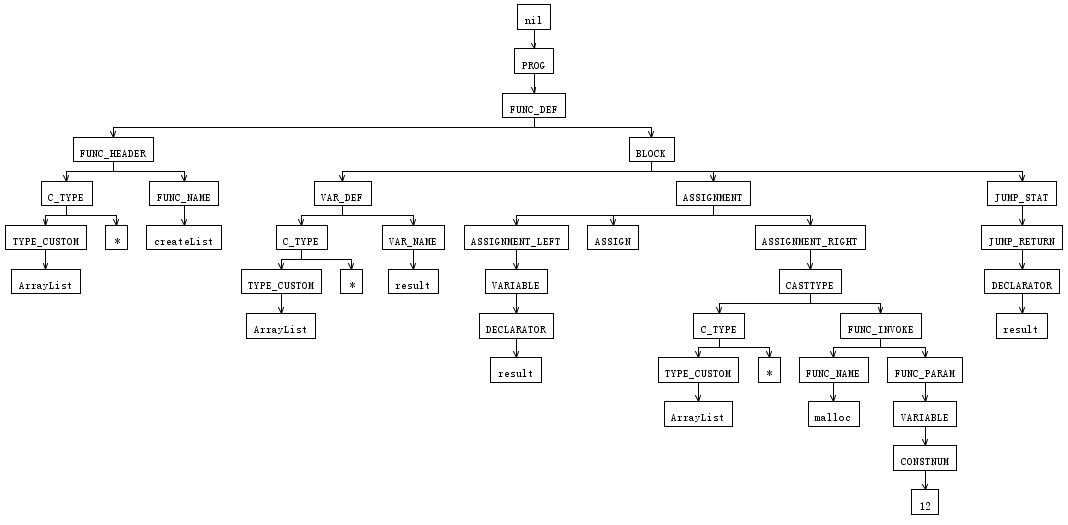
\includegraphics[width=6in]{ASTdemo.png}
    \end{center}
    
    \subsection{语法及语义检查}
    \subsubsection{实现概况}
    这部分应该遍历AST进行相应的检查,至少应包括变量、函数、类型等在内的不同标识符的作用域检查、函数参数列表检查等。考虑到每一种标识符的检查都是复杂繁琐的,由于时间有限,我们只对变量进行了作用域检查,其他的语法语义大同小异。

    \subsubsection{变量作用域检查}
    维护一张变量表paramTable,是普通的js对象,作为key-value映射表使用,以变量名作为key,而value则是该变量的作用域表。
    \par 每个变量的作用域表都是一个数组,其中填充布尔值,表示数组下标对应的作用域等级是否有该名称变量的定义,true表示有。
    \par 对于C语言的不同作用域,其作用域等级可能不同。全局作用域的作用域等级为1,每进入一个函数或一个BLOCK作用域(也就是大括号限定的作用域),作用域等级+1;每完成一个函数或BLOCK,释放该作用域的所有变量并恢复作用域等级。
    \par 当在特定作用域声明一个变量时,若该变量在当前作用域已经存在,就报错,形如:
    \begin{verbatim}
existed: ParamName
    \end{verbatim}
    \par 当在特定作用域中调用了一个变量时,若该变量在变量表中没有定义(如果某个变量释放后其对应的作用域表均为false,会删除该变量的作用域表,这样在变量表中没有定义的变量就是在当前作用域不可用的),就报错,形如:
    \begin{verbatim}
not found: ParamName
    \end{verbatim}

    \subsection{目标代码生成}
    \subsubsection{实现概况}
    前面我们已经完成了AST的构建并通过自顶向下的方式遍历AST完成了语法及语义的检查。到了目标代码生成阶段,虽然我们进行的语法及语义检查并不完善,但现在可以认为AST中不存在语法及语义错误,实际上在目标代码生成阶段就应该做这样的假设。
    \par 进行目标代码生成同样可以直接通过编写tree grammar来进行,但我们仍采用了手动遍历的方式进行,虽然增加了手动编码量,但减少了最终代码量,希望能以此提高效率。
    \par 经过努力,我们支持了在编译过程中保持大量语言特性,甚至已经拥有编译稍微复杂的C语言程序的能力。

    \subsubsection{自顶向下基于模板的目标代码生成}

    \subsubsection{目前支持的C语言特性}
    \begin{enumerate}
        \item 数据类型与变量
        \begin{enumerate}
            \item 支持结构体、数组、指针等;
            \item 但不支持指针的指针;
            \item 结构体成员也支持数组、指针等;
            \item 支持字符串常量;
            \item 支持整型常量;
            \item 支持局部变量(即非全局变量,也就是有一定作用域的变量)。
        \end{enumerate}
        
        \item 类型转换
        \begin{enumerate}
            \item 支持显式类型转换、隐式类型转换;
            \item 支持特殊的指针转整型:ptrtoint;
            \item 支持typedef。
        \end{enumerate}
        
        \item 函数
        \begin{enumerate}
            \item 支持函数定义、调用;
            \item 支持无返回值(void)的函数;
            \item 支持printf、malloc、free、memcpy等系统函数;
            \item 自动进行隐式类型转换。
        \end{enumerate}
        
        \item 运算
        \begin{enumerate}
            \item 赋值(会进行隐式类型转换);
            \item 支持加减乘除等常用算术运算;
            \item 自增(++)、自减(--);
            \item 支持常用逻辑运算。
        \end{enumerate}

        \item 选择语句
        \begin{enumerate}
            \item 支持;
            \item 还支持选择语句的嵌套(形如if...else{if...else...})。
        \end{enumerate}

        \item 循环语句:支持for和while。
    \end{enumerate}

    \subsection{自动化测试}
    \subsubsection{实现概况}
    完成了一个自动化测试实例C2LLVM/tests/test-main.js,运行方法见\ref{sec:abouttest}。 该测试中会读入arraylist.c文件,然后将目标代码输出至result.ll。这两个文件都放在C2LLVM/tests/data 目录下。

    \subsubsection{自动化测试步骤}
    在该自动化测试程序中,将语法文件名“SimpleCv4”作为参数创建一个C2LLVM编译器对象compiler,然后将测试文件的路径作为参数调用compiler的compile函数对此测试文件进行处理,返回值为目标代码的字符流result,最后将字符流result写到result.ll文件中,自动化测试结束。

    \section{实验结果}
    本实验提供的arraylist.c的解析结果见result.ll。
    \par arraylist.c中定义了结构体ArrayList,实现了创建、释放、扩增容量、插入数据、删除数据(两种方式:根据索引、根据值)、排序、功能测试等函数。在其中频繁进行选择判断、循环、函数调用等,其复杂性基本能说明我们的编译器已经对较复杂C语言程序有不错的支持。但其中有些地方仍按照奇怪的方式来书写,比如为了避免类似\lstinline{char *a, *b, c;}这样语句造成的处理难度,我们的编译器只支持\lstinline{char *a; char *b; char c;}这样的方式来定义变量。
    \par 值得一提的是,clang的编译结果(tests/data/arraylist.ll)为33KB,809行;而我们的编译结果(result.ll)为27KB,707行。实际上我们的编译器不会处理相同的字符串,而clang是处理了的,如果我们再加上处理相同字符串的功能,编译结果将能进一步缩减尺寸。
    \par 将result.ll在Linux环境下,用\lstinline[language=sh]{clang -o result result.ll} 将其编译为二进制文件,然后执行\lstinline[language=sh]{./result},输出结果如下。这与clang直接编译arraylist.c的结果表现一致。可以看到各个功能都被正确地执行了,特别是排序,涉及比较复杂的过程,这些正确的结果有理由让我们相信我们的编译结果是正确的。
    \begin{verbatim}
Start test ArrayList.

> Create an ArrayList.
>> Action: <empty>
>>> Returned: 0x9184008

> Initialize the ArrayList.
>> Action: list1.init()
>>> Returned: 0x0

> Create an ArrayList.
>> Action: <empty>
>>> Returned: 0x9184030

> Initialize the ArrayList.
>> Action: list2.init()
>>> Returned: 0x0

> Insert to the ArrayList.
>> Action: list1[0]=5
>>> Returned: 0x0

> Insert to the ArrayList.
>> Action: list1[1]=2
>>> Returned: 0x0

> Insert to the ArrayList.
>> Action: list1[2]=8
>>> Returned: 0x0

> Insert to the ArrayList.
>> Action: list1[3]=9
>>> Returned: 0x0

> Remove from the ArrayList by value
>> Action: list1.removeValue(9)
>>> Returned: 0x0

> Insert to the ArrayList.
>> Action: list1[3]=0
>>> Returned: 0x0

> Insert to the ArrayList.
>> Action: list1[4]=6
>>> Returned: 0x0

> Insert to the ArrayList.
>> Action: list2[0]=7
>>> Returned: 0x0

> Insert to the ArrayList.
>> Action: list2[0]=0
>>> Returned: 0x0

> Insert to the ArrayList.
>> Action: list2[0]=9
>>> Returned: 0x0

> Insert to the ArrayList.
>> Action: list2[0]=2
>>> Returned: 0x0

> Insert to the ArrayList.
>> Action: list2[0]=4
>>> Returned: 0x0

> Sort the combined ArrayList.
>> Action: list1.sort()
>>> Returned: 0x9184008

Sorted list1: 0 2 5 6 8

> Delete the ArrayList.
>> Action: list1
>>> Returned: 0x0

> Delete the ArrayList.
>> Action: list2
>>> Returned: 0x0
    \end{verbatim}

\clearpage
\end{CJK*}
\end{document}


